% !TeX root = ../thuthesis-example.tex

\chapter{实验与结果分析}
本节将会对第3章和第4章提出的时间序列对称子段判定和挖掘算法进行
实验验证和结果分析工作。
具体而言,主要包括对第3章提出的对称子段判定算法
进行结果对比和验证,对第4章提出的对称子段挖掘算法进行
效果和性能评估,并且对比了基于UDF和元数据的两种分段算法实现
的写入和查询性能。

\section{实验环境与对比方法}
本文实验所使用的环境如表~\ref{tab:experiment_enviroment}所示。
实验所使用的数据集,一方面来自UCR提供的时间序列数据集,
另一方面来自真实应用场景的时间序列数据。
UCR中每类数据集的时间序列长度都相同。
真实的数据集来自传感器采集的工业大数据,
其中每条时间序列都包含多个工况信息。
真实工业时间序列数据存在噪声、缺失和异常点等干扰,
对称子段挖掘有一定难度。
针对不同实验对于数据的要求,
本文选择合适的数据集进行实验,具体的数据集信息将在实验过程中
进行详述。

\begin{table}
  \centering
  \caption{实验环境介绍}
  \begin{tabular}{ll}
    \toprule
    实验环境     & 具体参数                          \\
    \midrule
    操作系统     & macOS 版本 10.15.5                \\
    处理器       & 2.4 GHz 四核Intel Core i5         \\
    内存         & 16 GB 2133 MHz LPDDR3             \\
    固态硬盘     & 256GB                             \\
    代码语言     & Python                            \\
    集成开发环境 & PyCharm 2020.1(Community Edition) \\
    \bottomrule
  \end{tabular}
  \label{tab:experiment_enviroment}
\end{table}

由于目前尚无成熟的对称子段挖掘方法,
为充分证明本文方法的准确性和高效性,
本章从对称性度量方式出发设置了两组基线算法作为对照方法,
其一为利用原始和反转时间序列相似性度量对称性的算法,
另一个是通过对称中心两侧子序列的相似性度量对称性的算法。
由于时间序列数据的连续性和不稳定性,不同类型时间序列数据的对称中心
不确定,因此,本文选用时间序列的几何中心作为其对称中心。
此外,正如2.4节所述,时间序列相似性度量算法种类多样,
仅基于形状的相似性度量算法就远不止一种。
若将时间序列视为多维空间中的点,
则其相似性度量本质上是度量多维数据点的距离。
相比适用于离散型变量的汉明距离和Jaccard距离与只利用一个维度信息的
切比雪夫距离,曼哈顿距离和欧氏距离分别通过计算
两段时间序列在高维空间的直线距离和多个维度的距离之和
来度量相似性,在不同来源的时序数据上具有更加通用的度量效果。
此外,曼哈顿距离和欧氏距离采用一一对应的方式度量时间序列的相似性,
而DTW算法和FastDTW算法则对时间序列进行全局匹配,
与本文提出的方法形成对照。
基于深度学习等数学模型度量时间序列相似性的方法
虽然可以通过降维实现快速检索,但由于变换产生的信息损失使得其
在实际度量效果中不如基于序列形状的算法。
因此,本文选择了包括基于
曼哈顿距离、欧氏距离、DTW距离和FastDTW距离在内的4种相似性
度量算法,其中每种算法都可以用来为对照组的两组算法提供相似性度量
计算。表~\ref{tab:experiment_algorithm}对本实验涉及到的9种时间序列
对称性度量算法进行了介绍。
由于不同度量算法的计算方式不同,不同数据集的时间序列长度
也不同,为了在同一量纲上进行比较,在通过表~\ref{tab:experiment_algorithm}
中的算法度量得到对称度之后,需要再计算其
与时间序列长度的比值得到单点对称度,作为最终统一衡量时间序列
对称性的值。
\begin{table}
  \centering
  \caption{实验算法介绍}
  \begin{tabular}{ll}
    \toprule
    算法名称          & 对称性度量方式                      \\
    \midrule
    symmetry          & 基于最优匹配策略                    \\
    manhattan         & 基于原始和反转时间序列的曼哈顿距离  \\
    euclidean         & 基于原始和反转时间序列的欧氏距离    \\
    dtw               & 基于原始和反转时间序列的DTW距离     \\
    fastdtw           & 基于原始和反转时间序列的FastDTW距离 \\
    center\_manhattan & 基于中心点两侧时间序列的曼哈顿距离  \\
    center\_euclidean & 基于中心点两侧时间序列的欧氏距离    \\
    center\_dtw       & 基于中心点两侧时间序列的DTW距离     \\
    center\_fastdtw   & 基于中心点两侧时间序列的FastDTW距离 \\
    \bottomrule
  \end{tabular}
  \label{tab:experiment_algorithm}
\end{table}

\section{对称子段判定效果评估实验}

由于时间序列子段的数据值是连续数据,
具有一定的随机性和波动性,不同于对称字符串,
现有研究中并不存在一个明确统一的对称性度量算法。
因此,本文基于时间序列子段的数据特征,提出了一种
基于区间动态规划和最优匹配的单一对称性度量算法。
为了检测对称性度量算法的效果,
本文在UCR数据集中选择了两个具有明显对称性的时间序列数据集
和两个不具有对称性的时间序列数据集,
这4个数据集的详细介绍如表~\ref{tab:experiment_dataset}所示。

在这4个数据集中,GunPointAgeSpan的时序数据表示
一套完整的持枪动作,而UMD的时间序列表示的是实验室信号合成数据,
两者都具有对称的物理意义。而GestureMidAirD1和MixedShapes
分别是手势轨迹和由普通二维形状转换而来的时间序列数据,
不具有对称性。分别对这两组包含正负样本的数据集进行实验,
可以验证本文对称性度量算法的有效性。为保证正负样本的数据
条数大致相同,不会出现数据倾斜问题,本文通过采样保证了
对称数据集和非对称数据集的时间序列条数均为147。

\begin{table}
  \centering
  \caption{对称子段判定算法实验数据集介绍}
  \begin{tabular}{ccccc}
    \toprule
    数据集名称      & 来源         & 类型 & 数据条数 & 长度 \\
    \midrule
    GestureMidAirD1 & 3D手势轨迹   & 运动 & 47       & 361  \\
    GunPointAgeSpan & 完整举枪动作 & 运动 & 135      & 150  \\
    MixedShapes     & 二维形状转换 & 图像 & 100      & 1024 \\
    UMD             & 信号合成     & 模拟 & 12       & 150  \\
    \bottomrule
  \end{tabular}
  \label{tab:experiment_dataset}
\end{table}

首先在对称数据集上进行对称子段判定实验,分析不同数据集
时间序列的对称度结果,以及对称度阈值对对称子段判定的影响。
图~\ref{fig:symmetry_compare}展示了在两个对称数据集上,
不同对称性度量算法计算得到的对称度结果。经过对比可以发现,
本文所提出的子段对称性度量算法(symmetry算法)
计算得到的对称度总是最小的,
不仅小于基于原始和反转时间序列的相似性度量对称性的算法,
也小于基于中心点两侧时间序列相似性度量对称性的算法。
对于相同的对称度阈值,本算法可以挖掘出数量尽可能多的
对称子段。除此之外,从本结果中还可以看出,
尽管GunPointAgeSpan和UMD数据集的时间序列具有物理意义上
的对称性,而且时间序列的长度相同,
但其对称度的分布范围仍然相差甚大。以symmetry算法为例,在
GunPointAgeSpan数据集上度量135条时间序列得到的平均对称度
是3.846,而在UMD数据集上度量12条时间序列得到的平均对称度
仅为0.006,不同来源的数据集因为数据特征的差别其对称度阈值
差距较大,这为对称子段的判定也带来了困难,
从侧面证明了本文提出的对称度阈值算法的重要性。
\begin{figure}
  \centering
  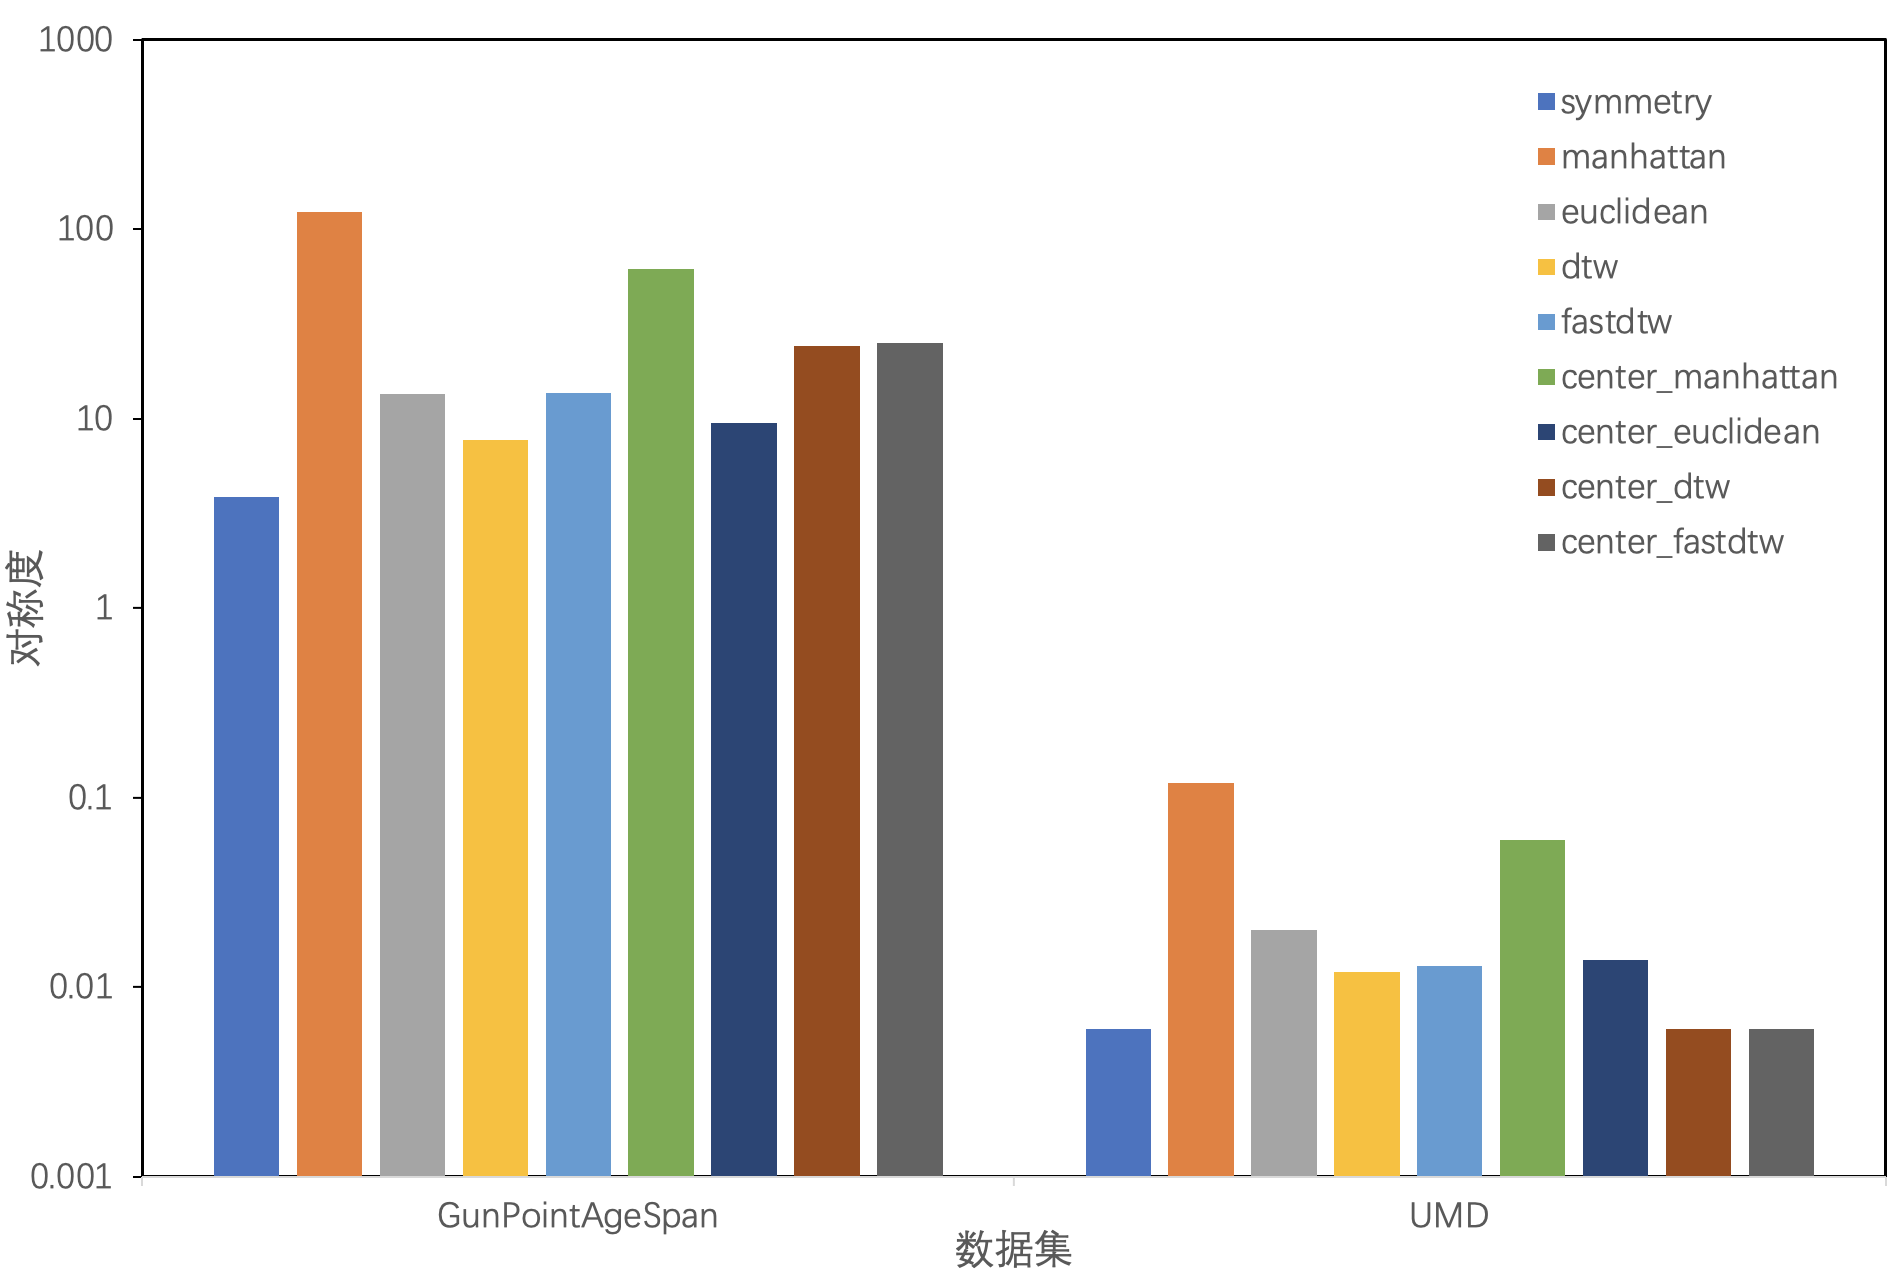
\includegraphics[width=0.76\linewidth]{symmetric_dataset_symmetry.PNG}
  \caption{对称数据集上不同算法的子段对称性度量结果}
  \label{fig:symmetry_compare}
\end{figure}

在真实的工业领域,往往采用领域专家指定对称度阈值的方式过滤对称子段。
因此,本文在GunPointAgeSpan和UMD这两个具有对称性的数据集上进行实验,
在计算得到数据集中时间序列的对称度之后,通过调整对称度阈值,
分析对称子段的判定效果。为保证在GunPointAgeSpan和UMD数据集
分别选择合适的对称度阈值变化范围
,本文通过统计每个数据集上所有时间序列
相邻点距离的最小值和最大值作为对称度阈值的变化范围。
图~\ref{fig:symmetry_heatmap}展示了当对称度阈值
发生变化时,对称子段判定效果随之发生的变化。其中,
使用对称中心度量对称性的算法用前缀c加以区分。
从图中可以看出两点:
\begin{enumerate}
  \item 尽管同为对称数据集,不同来源的时间序列变化
        剧烈程度不同,数据的差异程度也不同。
        GunPointAgeSpan数据集相邻点之间的距离最大可达327.48,
        而UMD数据集相邻点之间的距离最大仅为0.42,
        不利于领域专家人为确定对称度阈值。结合图~\ref{fig:symmetry_compare}
        关于GunPointAgeSpan和UMD数据集对称度度量结果的比较,发现时间序列相邻点变化剧烈的
        数据集,其对称度也偏大,对称度和时间序列相邻点距离呈正相关。
        因此,基于时间序列
        数据特征确定对称度阈值的算法是可行的。
  \item 随着对称度阈值的增大,对称子段判定算法很快收敛,能挖掘出
        对称数据集GunPointAgeSpan和UMD中所有的对称子段。
        同样,基于DTW距离的
        对称性度量方法也较快收敛。
        但是,基于一一对应和对称中心的算法
        却需要较高
        的对称度阈值才能挖掘出数据集中所有的对称子段。
        甚至在GunPointAgeSpan数据集中,manhattan算法在
        对称度阈值达到200时仍然只能挖掘出低于60\%的对称子段。
        证明了相比一一对应,基于最优匹配
        的对称性度量算法在对称子段判定具有更好的稳定性。

\end{enumerate}
\begin{figure}
  \centering
  \subcaptionbox{GunPointAgeSpan\label{fig:gun_heatmap}}
  {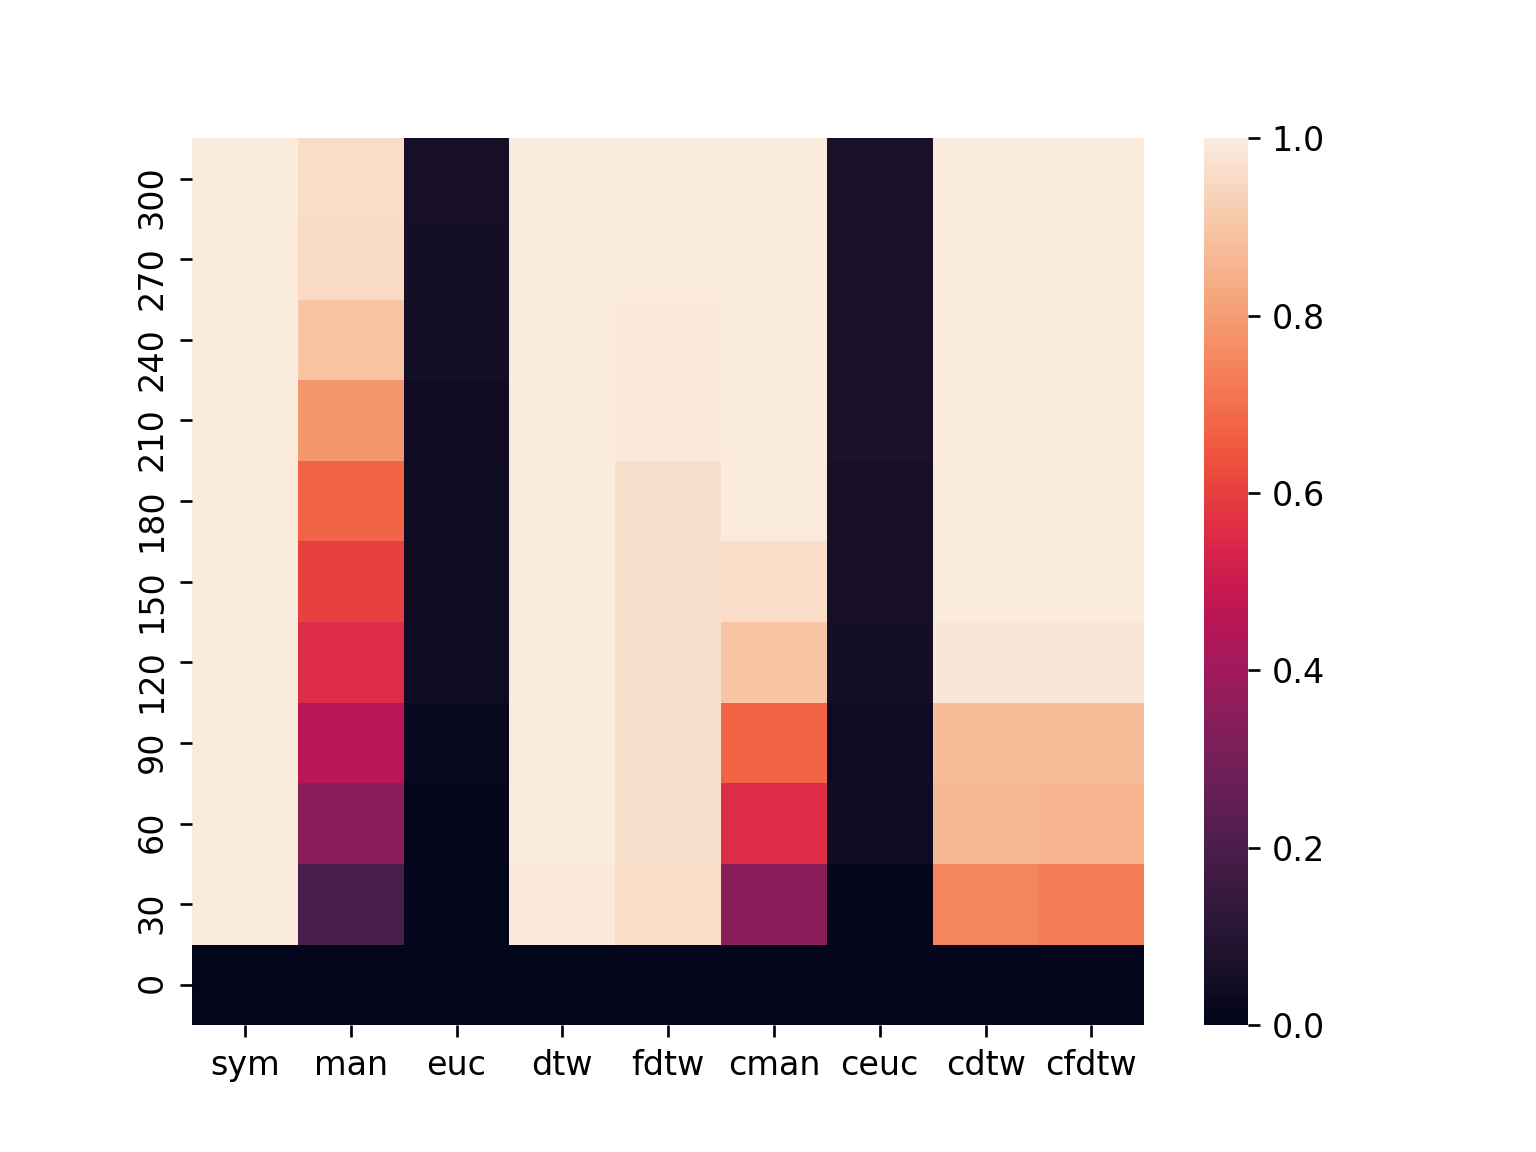
\includegraphics[width=0.49\linewidth]{gun_heatmap.png}}
  \subcaptionbox{UMD\label{fig:umd_heatmap}}
  {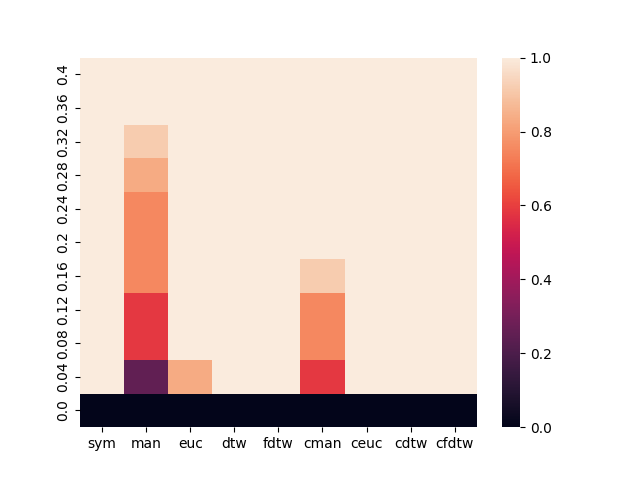
\includegraphics[width=0.49\linewidth]{umd_heatmap.png}}
  \caption{不同对称度阈值下对称子段判定效果}
  \label{fig:symmetry_heatmap}
\end{figure}

由于不同来源的时间序列数据特征差别很大,
采用领域专家直接指定对称度阈值的方式在处理不同来源的数据集时并不现实。
本文使用相邻点之间的距离作为匹配点之间
的距离阈值参考,进而得到单一对称度阈值,以进行对称子段的
判定。接下来本文将对表~\ref{tab:experiment_dataset}中所示
的4个数据集进行对称子段判定算法的效果实验,
并利用准确率,精确率,召回率和F值综合评价挖掘效果。在这4个数据集中,GunPointAgeSpan和UMD数据集
具有对称性,而MixedShapes和GestureMidAirD1数据集没有对称性。
在实验过程中,本文把对称子段标记为正类(positive),把非对称子段标为负类(negative)。
当算法在对称数据集中发现对称子段时,这类时间序列用TP表示。当算法
在对称数据集中发现非对称子段时,这类时间序列用FN表示。当算法
在非对称数据集中发现对称子段时,这类时间序列用FP表示。当算法
在非对称数据集中发现非对称子段时,这类时间序列用TN表示。
基于以上四类情况,可以定义时间序列对称子段判定算法的
准确率(Accuracy),精确率(Precision)和召回率(Recall)和F值。
其中,准确率表示挖掘正确的样本数和总样本数的比值。
准确率是最为常见的一类效果统计指标。
式~\ref{eq:precision}表示了精确率的计算方式。
精确率又叫查准率,定义为在所有被预测为正的样本中,
实际为正样本的概率,在本实验中的含义是预测为对称子段的时间序列中有多少是真正的对称时间序列,
式~\ref{eq:precision}表示了精确率的计算方式。召回率又叫查全率,定义为在所有真实为正
的样本中,预测为正样本的概率,在本实验中的含义是
真实为对称子段的时间序列中有多少被预测为了对称时间序列。
式~\ref{eq:recall}表示了召回率的计算方式。F值的定义是准确率和召回率的加权平均数,
为平衡准确率和召回率,本文选择F1值作为F值度量结果,式~\ref{eq:f1}表示了
F1值的计算方式。
\begin{equation}
  Accuracy=\frac{TP+TN}{TP+FP+TP+TN}
  \label{eq:Accuracy}
\end{equation}
\begin{equation}
  Precision=\frac{TP}{TP+FP}
  \label{eq:precision}
\end{equation}
\begin{equation}
  Recall=\frac{TP}{TP+FN}
  \label{eq:recall}
\end{equation}
\begin{equation}
  F1=\frac{2 \times Precision \times Recall}{Precision+Recall}
  \label{eq:f1}
\end{equation}

准确率十分直观地展示了不同算法对称子段判定的效果。
图~\ref{fig:accuracy_compare}即为不同算法挖掘对称子段
准确率的对比结果。从图中可以很明显地看出,
symmetry算法判定对称子段的准确率远高于其他算法。
即便是同样采用全局匹配的基于DTW和FastDTW距离的对称子段判定算法,
其准确率也低于symmetry算法。
除此之外,从图中还可以对比得到,
对称子段判定准确率和对称中心的明确与否关系不大,
与子段对称性的度量方式关系很大。
不管对称中心是否明确,对称子段判定准确率由高到低依次为
symmetry算法、基于DTW或FastDTW距离的算法、
基于欧氏距离的算法和基于
曼哈顿距离的算法。其中准确率最低的
基于曼哈顿距离的判定算法几乎只能识别对一半
的对称子段,在实验数据集样本均衡的前提下,其准确率与随机猜测已差别不大,
几乎不具有实用价值。这证明了本文提出的基于最优匹配的对称性度量算法
的有效性。
\begin{figure}
  \centering
  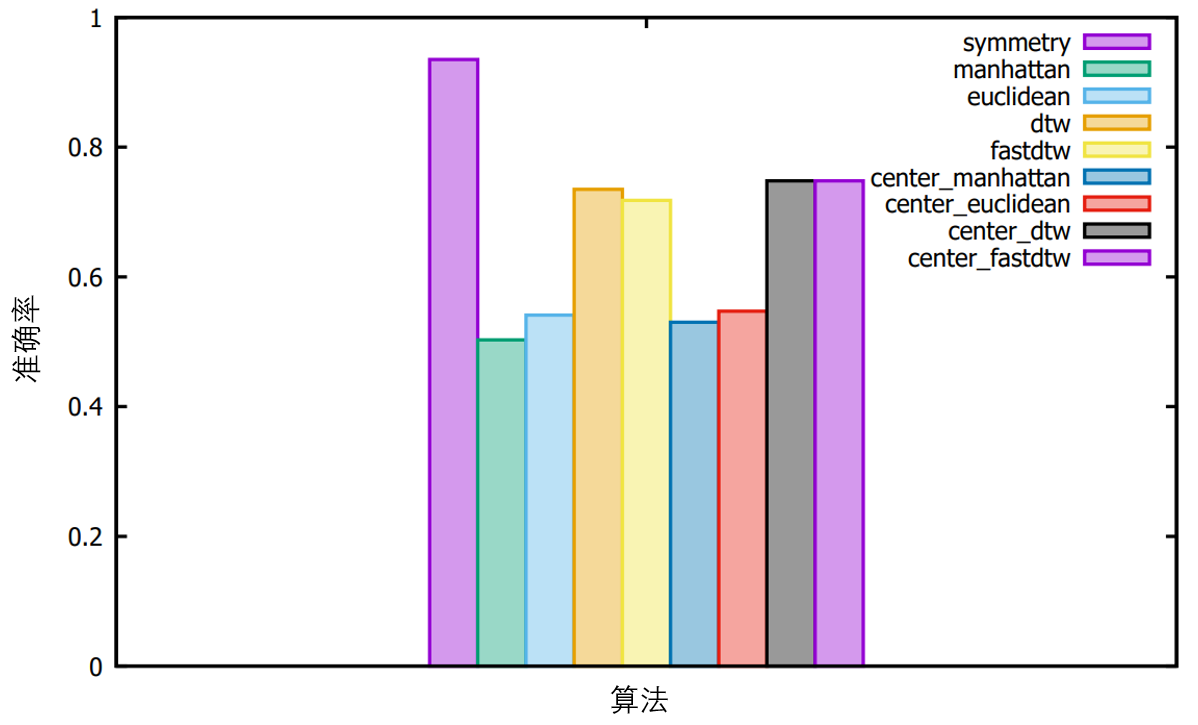
\includegraphics[width=0.76\linewidth]{symmetry_accuracy.PNG}
  \caption{不同对称子段判定算法的准确率结果}
  \label{fig:accuracy_compare}
\end{figure}

尽管准确率十分直观地度量了时间序列对称子段判定的效果,
但由于其过于简单,易受到实验数据集的影响。
为了综合评价算法的挖掘效果,本文选用F值表示算法的对称子段判定效果。
因为精确率是判定出的对称子段中真正对称子段所占的比例,表示了
算法判定对称子段的准确程度。而召回率是对称数据集中判定出对称子段
所占的比例,衡量了算法对于对称子段的识别能力,召回率越高,表明算法
能挖掘出更全面的对称子段。很明显,精确率和召回率是两个
冲突的指标。精确率是关于算法挖掘准确性的度量,召回率是关于算法挖掘覆盖面的
度量。一个优秀的算法应该同时具有较高的精确率和召回率。
F值就是用来综合评估算法的精确率和召回率。在实验中,本文采用F1值度量
模型效果的优劣。图~\ref{fig:fscore_compare}展示了在表~\ref{tab:experiment_dataset}
所示的数据集下进行对称子段判定,不同F值的结果。从图中可以发现,symmetry
算法的F值要远高于其他算法,证明了对称子段判定算法的有效性。

\begin{figure}[t]
  \centering
  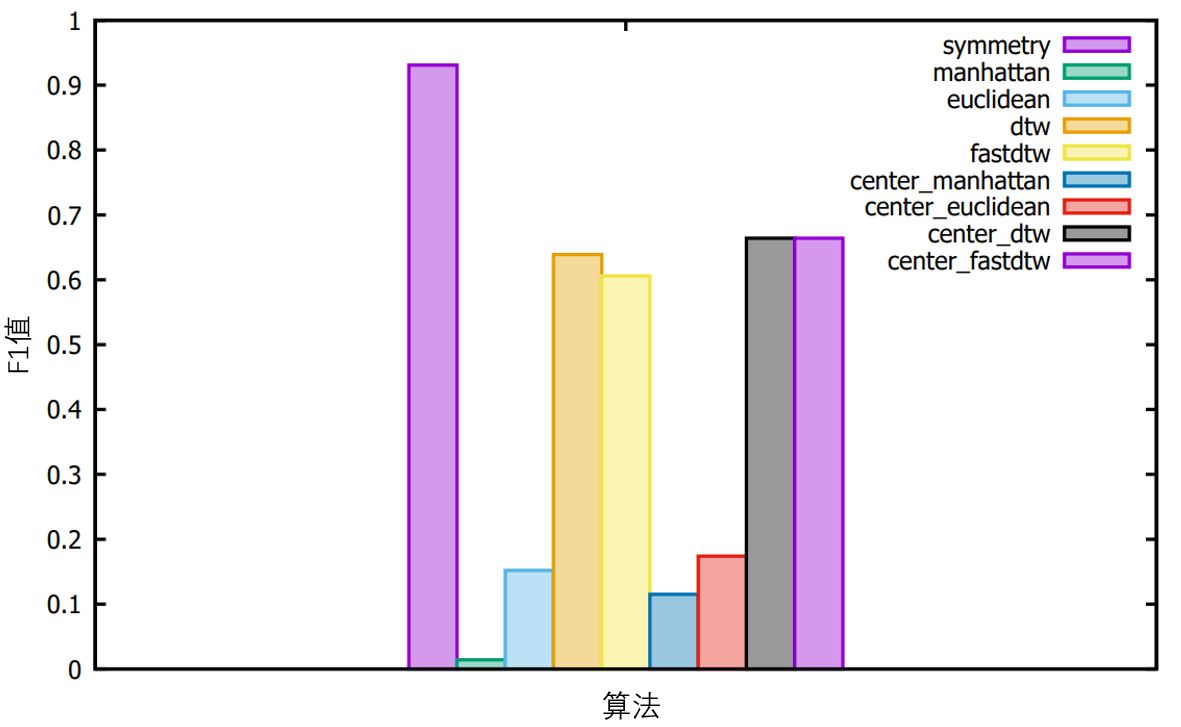
\includegraphics[width=0.76\linewidth]{f-score.PNG}
  \caption{不同对称子段判定算法的F1值结果}
  \label{fig:fscore_compare}
\end{figure}

\begin{table}
  \centering
  \caption{不同算法对称子段判定效果评估}
  \begin{tabular}{llll}
    \toprule
    算法              & Precision & Recall & F-score \\
    \midrule
    symmetry          & 1.0       & 0.871  & 0.931   \\
    manhattan         & 1.0       & 0.007  & 0.014   \\
    euclidean         & 0.872       & 0.232  & 0.366   \\
    dtw               & 1.0       & 0.469  & 0.639   \\
    fastdtw           & 1.0       & 0.435  & 0.606   \\
    center\_manhattan & 1.0       & 0.061  & 0.115   \\
    center\_euclidean & 0.726       & 0.306  & 0.431   \\
    center\_dtw       & 1.0       & 0.497  & 0.664   \\
    center\_fastdtw   & 1.0       & 0.497  & 0.664   \\
    \bottomrule
  \end{tabular}
  \label{tab:experiment_global_algo}
\end{table}

为了更细致的分析不同算法F值差别的原因,表~\ref{tab:experiment_global_algo}
列出了实验对比所有算法的精确率,召回率和F值。观察表格发现,
symmetry算法的召回率非常高,几乎是基于DTW距离的对称性度量算法
的两倍,证明了symmetry算法在不同数据集上判定对称子段的全面性,
能挖掘出尽可能多的对称子段。
而基于欧氏距离和曼哈顿距离的对称性度量算法,由于采取一一对应
的匹配方式,忽略了时间序列在不同阶段的采样率和持续时间不同,
其召回率非常低。
除此之外,对称子段判定算法采用基于时间序列数据特征的相邻点距离均值
作为对称度阈值。由于算法能为不同来源的数据集确定合适的对称度阈值,
因此所有对称子段判定算法的精确率都非常高。

\section{对称子段挖掘算法实验}

5.2节对对称子段判定算法进行了效果评估实验。除了
要判定子段的对称性,更多的对称子段嵌入在
长时间序列之中,需要采用对称子段挖掘算法对其进行挖掘。
本文采用了1个人工合成数据集和3个真实工业数据集,
具体的数据信息如表~\ref{tab:segment_dataset}中所示。
其中,人工合成数据集由30000个点组成,
除部分噪声影响之外,原始数据为以360个点为一个完整周期的
正弦函数采样数据。
真实工业数据集1来源于GPS轨迹数据,包含33500个点。
主要采集了运输车运输货物行驶轨迹形成的GPS信息,
每一趟GPS轨迹信息具有物理上的对称性。由于车速
和运输路线的不同,运输车运输一趟的
平均时间为 30 分钟,最长为 48 分钟。
真实工业数据集2为等时间间隔采样的挖掘机挖斗数据,
共35189个数据点。
主要采集了挖掘机在挖掘过程中各个工况的变化,
挖掘机作业形成的工况时间序列也具有分段对称性。
但由于挖掘机每次挖掘的坑道不一致,且两次作业间存在等
待期,导致挖掘机工况对称子段持续的时间长度变化较大。
真实工业数据集3为上证指数2016年至2019年以天为单位变化
的时间序列,共有3186个数据点。
由于股票数据具有长期增长的趋势性特征,其对称子段出现较少,
可通过人工标注对称子段作为正确结果。
实验采用的4个数据集各有特点:
人工数据集具有明显的周期性;运输车轨迹数据集运行时间较长,
对称性较为明显;挖掘机工况数据集对称子段较长,噪声也较多,
对称性不易挖掘;上证指数数据集对称子子段非常少,持续时间同样很长。
若算法在这4类数据集上的表现均比较良好,
则证明了对称子段挖掘算法的有效性。

\begin{table}
  \centering
  \caption{对称子段挖掘算法实验数据集介绍}
  \begin{tabular}{llll}
    \toprule
    数据集名称    & 来源               & 时间序列长度 \\
    \midrule
    合成数据集    & 正弦函数曲线       & 30000        \\
    GPS轨迹数据集 & 运输车轨迹信息     & 33500        \\
    工况数据集    & 挖掘机作业工况信息 & 35189        \\
    金融数据集    & 上证指数历年变化   & 3186         \\
    \bottomrule
  \end{tabular}
  \label{tab:segment_dataset}
\end{table}

\subsection{对称子段挖掘算法效果和性能评估}

对于总点数和对称子段长度约束不同的时间序列,
需要设定一个评价标准验证对称子段挖掘算法的效果。
虽然时间序列子段包含的数据点个数或多或少,
但是给定时间序列中子段的个数通常是固定的。
因此,本文采用对称子段的数量偏差评价真实结果和挖掘结果的相近程度。
式~\ref{eq:variation}展示了偏差率$\delta$的计算方式。
令$r_{truth}$作为时间序列对称子段的真实数量,
$r_{cal}$作为挖掘出的时间序列对称子段的数量。
则用$\delta$评估挖掘结果和真实结果的相似程度,表示挖掘效果
的误差率。$\delta$越小,说明挖掘结果越精确。偏差率$\delta$
作为算法的评价指标同样具有应用价值,实际工业场景中常有
统计对称子段数量的需求,例如挖掘机通过一天内的运输趟数记工打卡,
偏差率表示挖掘的运输趟数和真实运输趟数之间的差距,是算法优劣的重要指标。

\begin{equation}
  \delta \left( r_{truth}, r_{cal} \right) = \frac{\left| r_{cal} - r_{truth} \right|}{r_{truth}}
  \label{eq:variation}
\end{equation}

合成数据集,GPS轨迹数据集和工况数据集以秒或者毫秒为单位采集数据,
时间序列长,具有物理意义的对称子段较多,因此,本文在
长度由3000到30000不等的数据量上进行对称子段挖掘实验。
而金融数据集以天为单位采集数据,
时间序列长度和对称子段数量均较小,因而
本文在长度由600到3000不等的数据量上对金融数据进行
对称子段挖掘实验。
图~\ref{fig:segement_symmetry}展示了在这4个数据集上进行对称子段挖掘的效果。
首先是具有严格对称性的合成数据集,由图~\ref{fig:sin_1}和~\ref{fig:sin_2}
可知,除了manhattan算法效果较差之外,其他算法的效果均十分稳定。
分析算法可以得知,当对称子段长度约束设为360时,manhattan算法
以一一对应的方式计算对称度。尽管对称子段只有360个点,但在全部时间序列中
与子段第1个点对应的是下一个子段的第1个点,即第361个点。因此,
manhattan算法会在匹配点计算时产生偏差。
而由于正弦时间序列整体平稳,分段算法确定的对称度阈值也较小,因此其对称子段挖掘效果出现抖动,
当对称度阈值过小时,对称子段无法挖掘。
GPS轨迹没有明确的对称中心,其数据点也由于车辆行驶过程的随机性和采样
传感器的不精确而具有随机误差,同时,对称子段的长度也不固定。
为保证挖掘效果,本文采用车辆单趟运输轨迹的数据点采样个数最小值300作为长度约束挖掘对称子段。
由图~\ref{fig:truck_1}和~\ref{fig:truck_2}可知,symmetry算法的偏差率在所有算法中
处于最低水平,表明其挖掘出的对称子段数量和
真实结果最为接近,不仅远超过基于欧氏距离和曼哈顿距离的对称子段挖掘算法,也优于
DTW和FastDTW方法。
在所有方法中,仅有center\_DTW和center\_FastDTW算法和symmetry算法效果较为接近,但也略有不如
。证明对称子段挖掘算法具有很高的鲁棒性,在存在误差的数据集中
也能挖掘出正确的对称子段。

图~\ref{fig:excavator_1}和图~\ref{fig:excavator_2}是在挖掘机工况数据集
上进行实验得到的结果。挖掘机一次作业过程的时间序列
具有对称性,但是挖掘机作业过程中间歇阶段较多,作业类型不一致导致对称子段长度不固定,
且伴生着随机噪声和误差,使得对称子段挖掘任务更为复杂。
尽管如此,symmetry算法仍然将偏差率控制在了0.2以下,且随着
时间序列长度的增加,对称子段挖掘效果逐渐收敛,并无明显下降。
相比之下,基于欧氏距离和曼哈顿距离的对称子段挖掘算法不仅偏差率
较高,而且随时间序列的长度增加,起伏变化不定,稳定性很差。而基于DTW
距离和FastDTW距离的算法其效果也要差于symmetry算法。
金融数据集来源于上证指数10年内的数值变化,金融领域的数据具有很强
的实时性,短期内变化大,对称性不明显。在全局时间序列中,只存在两个局部的
对称子段。图~\ref{fig:stock_1}和图~\ref{fig:stock_2}展示了
在金融数据集上不同算法挖掘对称子段的偏差率,
从图中可知,基于DTW和FastDTW距离的算法在金融数据集上出现了性能的严重下降,
DTW和FastDTW方法甚至没有挖掘出一个对称子段。相比之下,symmetry算法的
效果保持稳定,在不同规模的时间序列中均挖掘出了正确数量的对称子段。
% 此外,center\_euclidean算法挖掘对称子段的效果和symmetry算法平齐,
% 分析算法发现,金融数据集单日变化过于剧烈,导致对称度阈值计算结果偏大,
% 间接提升了包括center\_euclidean在内的对称性度量结果较大
% 算法的子段挖掘效果。

总之,通过在不同来源的数据集上对不同算法进行对比实验综合发现:
\begin{enumerate}
  \item 从合成数据集、运输车GPS数据集到
        挖掘机工况数据集和金融数据集,对称子段的数量逐渐减少,数据偏差、失配、
        不对齐和噪声干扰逐渐增多,对称子段挖掘的难度不断增大。但是在所有数据集上,
        对称子段挖掘算法均有最优的表现。
  \item 同对称子段判定算法一样,基于一一对应的匹配方式
        在对称子段挖掘任务上同样表现较差,远低于基于时间扭曲和最优匹配
        的方法,从而导致对称子段的挖掘效果较差。
\end{enumerate}


\begin{figure}
  \centering
  \subcaptionbox{合成数据集\label{fig:sin_1}}
  {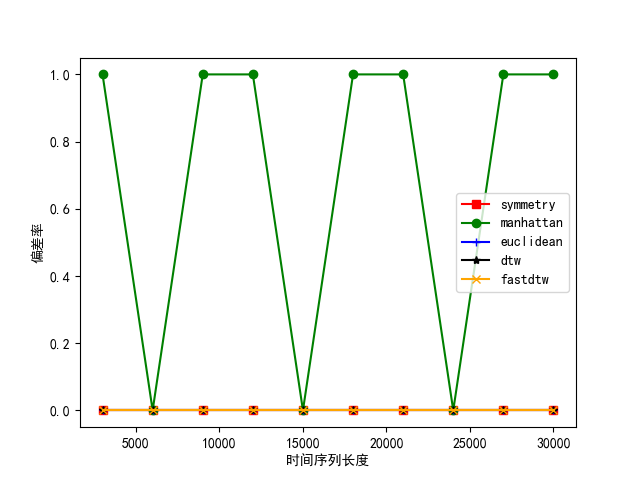
\includegraphics[width=0.43\linewidth]{sin_1.png}}
  \subcaptionbox{合成数据集\label{fig:sin_2}}
  {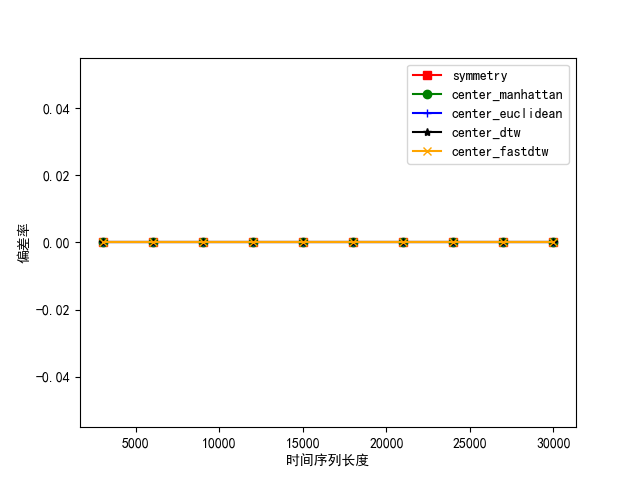
\includegraphics[width=0.43\linewidth]{sin_2.png}}
  \subcaptionbox{GPS轨迹数据集\label{fig:truck_1}}
  {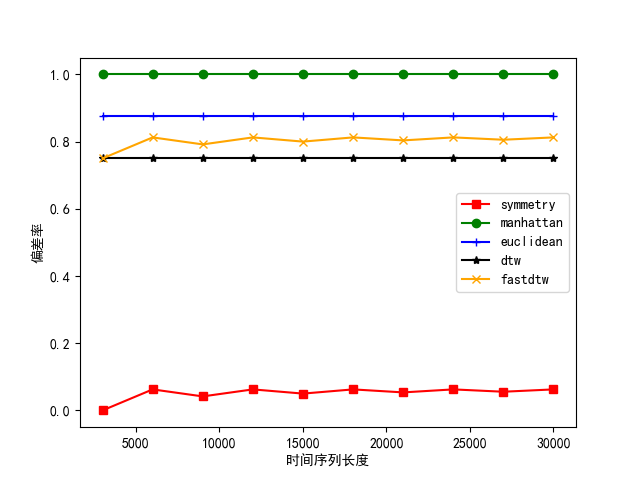
\includegraphics[width=0.43\linewidth]{truck_1.png}}
  \subcaptionbox{GPS轨迹数据集\label{fig:truck_2}}
  {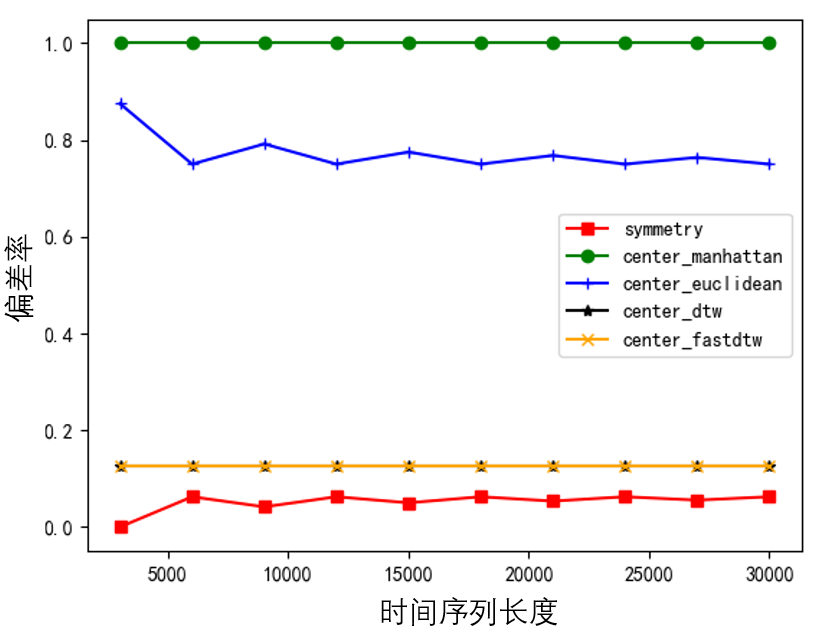
\includegraphics[width=0.43\linewidth]{truck_2.png}}
  \subcaptionbox{工况数据集\label{fig:excavator_1}}
  {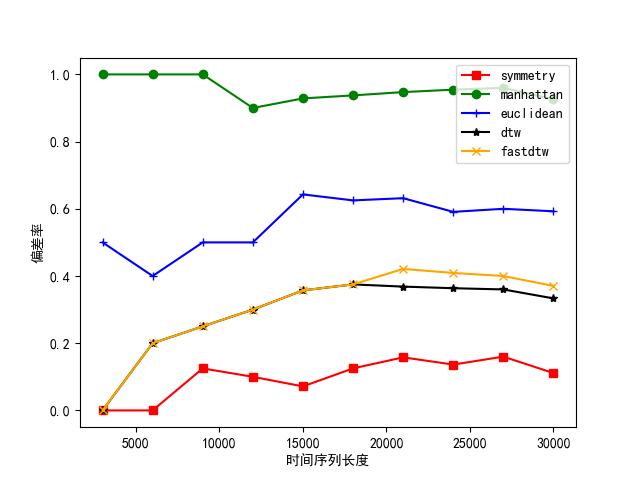
\includegraphics[width=0.43\linewidth]{excavator_1.png}}
  \subcaptionbox{工况数据集\label{fig:excavator_2}}
  {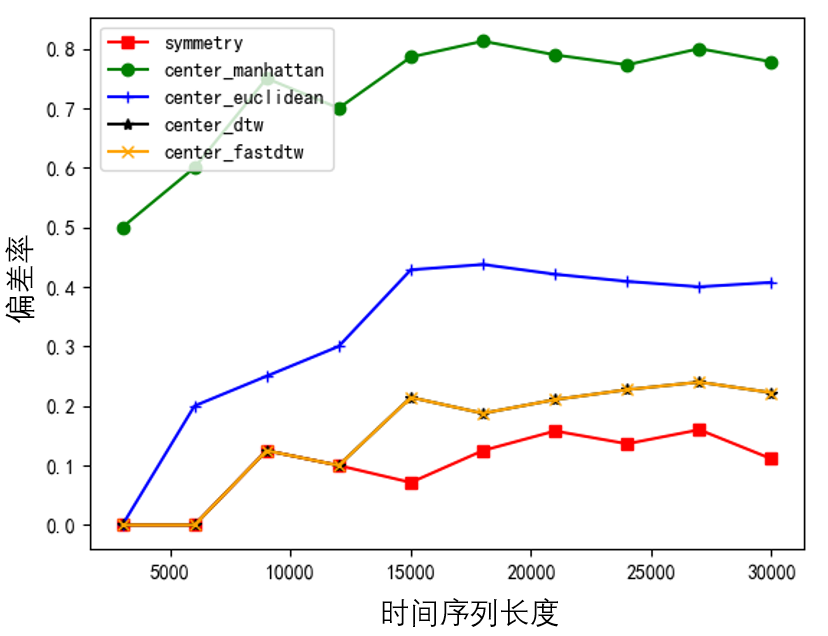
\includegraphics[width=0.43\linewidth]{excavator_2.png}}
  \subcaptionbox{金融数据集\label{fig:stock_1}}
  {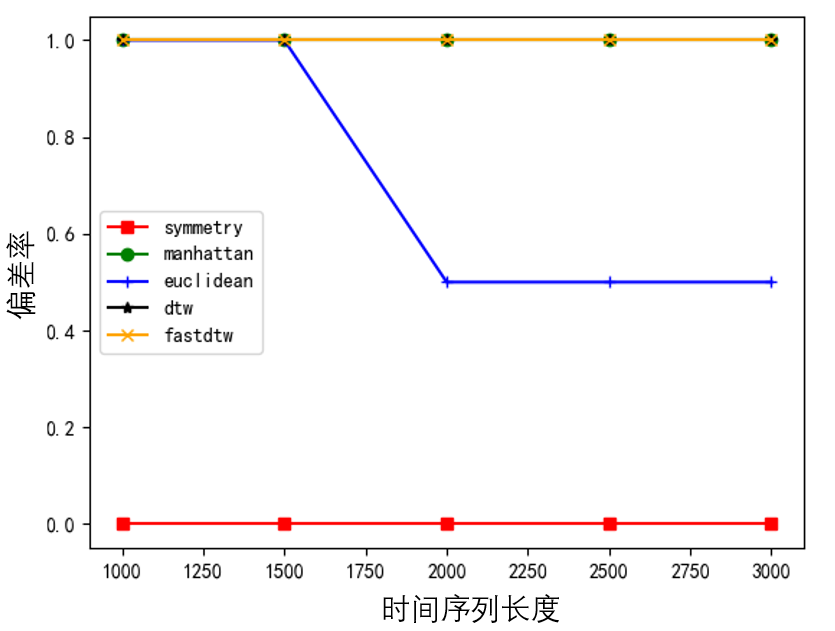
\includegraphics[width=0.43\linewidth]{stock_1.png}}
  \subcaptionbox{金融数据集\label{fig:stock_2}}
  {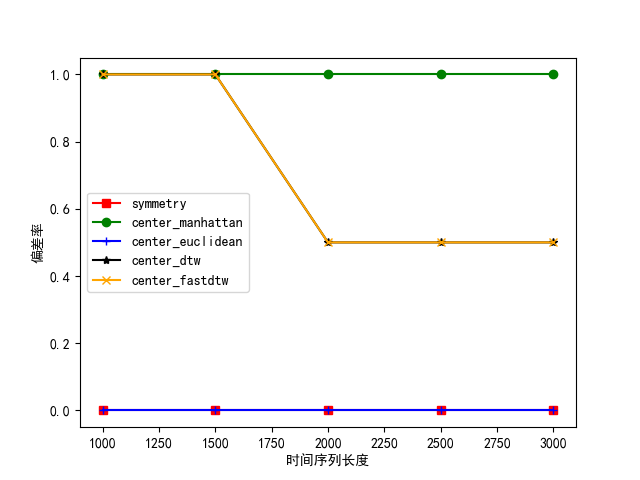
\includegraphics[width=0.43\linewidth]{stock_2.png}}
  \caption{对称子段挖掘偏差率对比}
  \label{fig:segement_symmetry}
\end{figure}

\begin{figure}
  \centering
  \subcaptionbox{合成数据集\label{fig:sin_time_1}}
  {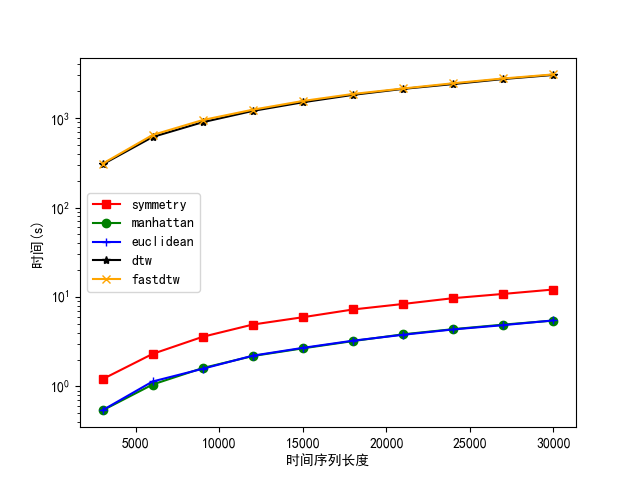
\includegraphics[width=0.43\linewidth]{sin_time_1.png}}
  \subcaptionbox{合成数据集\label{fig:sin_time_2}}
  {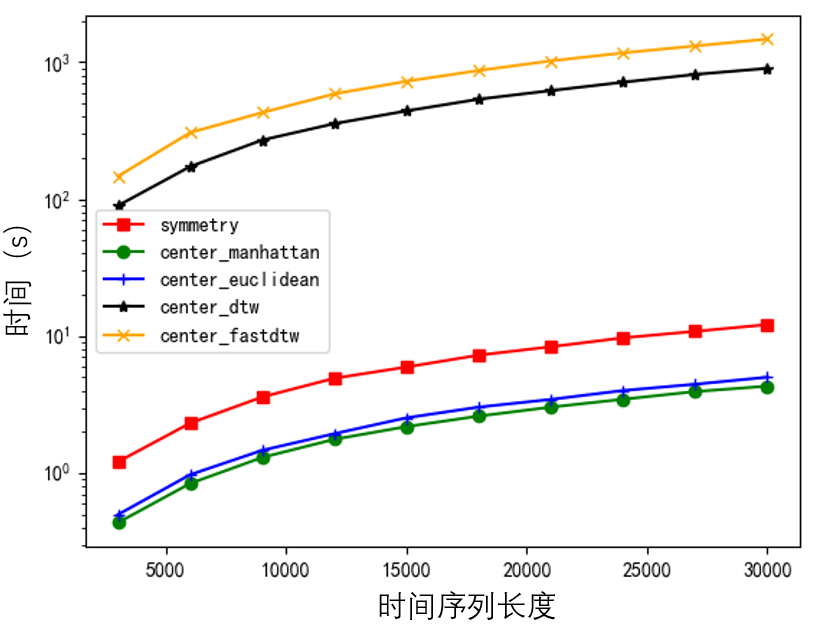
\includegraphics[width=0.43\linewidth]{sin_time_2.png}}
  \subcaptionbox{GPS轨迹数据集\label{fig:truck_time_1}}
  {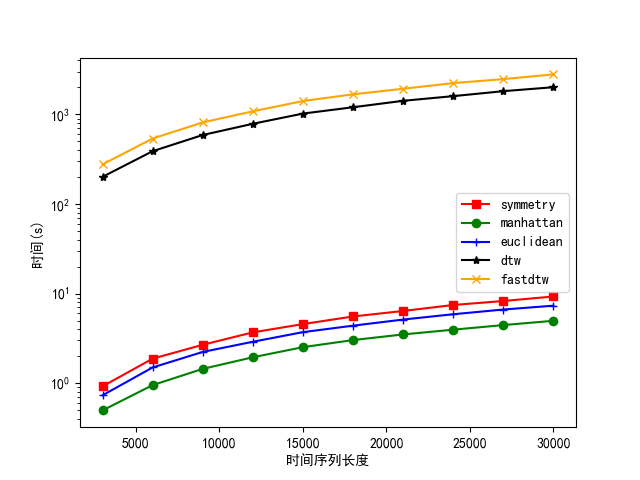
\includegraphics[width=0.43\linewidth]{truck_time_1.png}}
  \subcaptionbox{GPS轨迹数据集\label{fig:truck_time_2}}
  {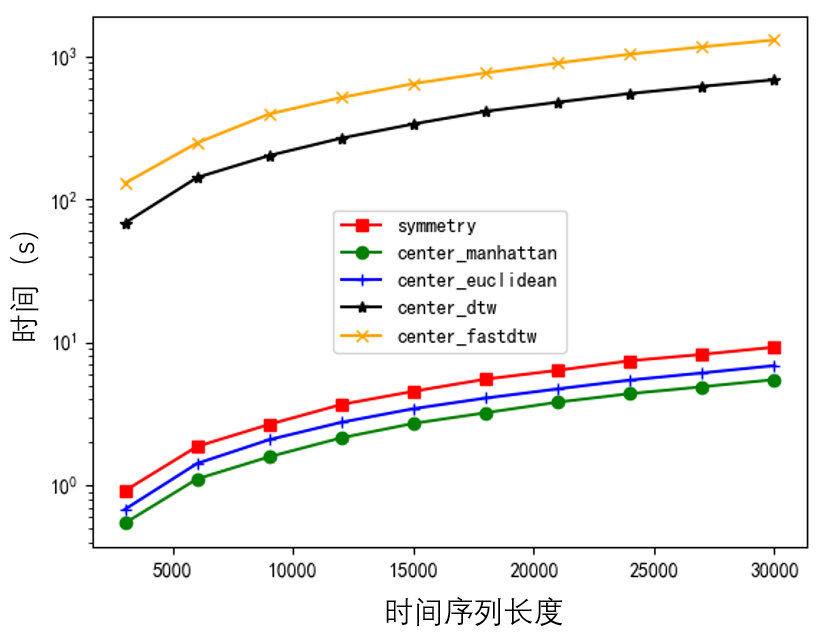
\includegraphics[width=0.43\linewidth]{truck_time_2.png}}
  \subcaptionbox{工况数据集\label{fig:excavator_time_1}}
  {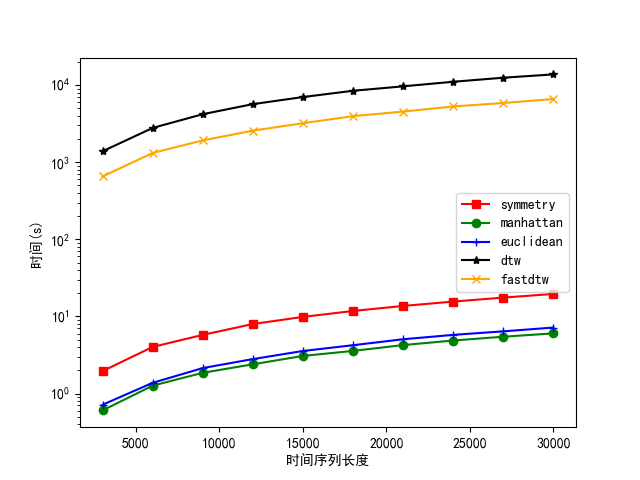
\includegraphics[width=0.43\linewidth]{excavator_time_1.png}}
  \subcaptionbox{工况数据集\label{fig:excavator_time_2}}
  {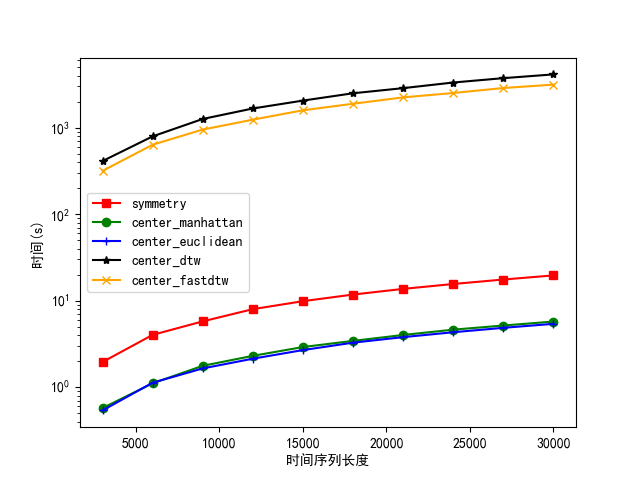
\includegraphics[width=0.43\linewidth]{excavator_time_2.png}}
  \subcaptionbox{金融数据集\label{fig:stock_time_1}}
  {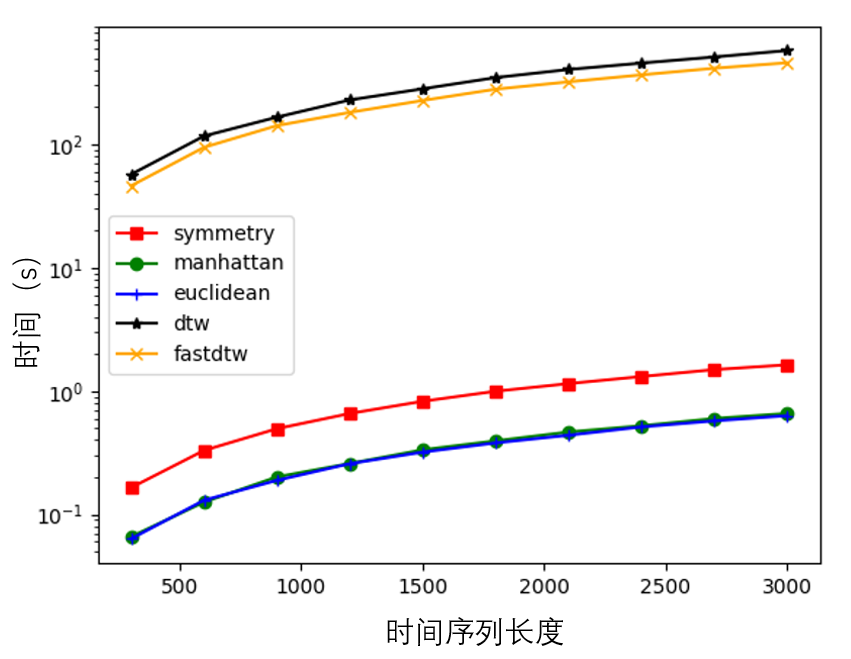
\includegraphics[width=0.43\linewidth]{stock_time_1.png}}
  \subcaptionbox{金融数据集\label{fig:stock_time_2}}
  {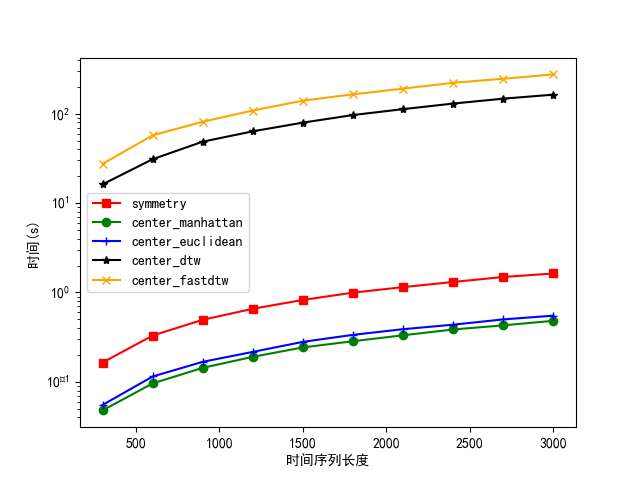
\includegraphics[width=0.43\linewidth]{stock_time_2.png}}
  \caption{对称子段挖掘时间效率对比}
  \label{fig:segement_algorithm_time}
\end{figure}

除了比较不同算法挖掘对称子段的效果,本文还对算法的时间性能进行了实验对比。
图~\ref{fig:segement_algorithm_time}展示了所有算法在不同数据集上
随时间序列长度增加而产生的时间开销变化。从图中可以很明显地看出,
对称子段挖掘算法的时间效率非常高,十分接近基于曼哈顿距离
和欧氏距离的挖掘方法,而远高于基于DTW距离的方法。
经过对算法复杂度的推导证明,对称子段挖掘算法的渐进时间复杂度
为$O\left(n \times w\right)$,而基于DTW距离的挖掘方法
其时间复杂度为$O\left(n \times w^2\right)$。算法时间性能的实验结果证明
了复杂度推导得到的结论。此外,对比图~\ref{fig:excavator_time_1}
和图~\ref{fig:truck_time_1}可知,时间序列的长度变化并不会影响算法
的相对性能,影响算法性能的因素主要是子段长度约束的大小。
基于DTW距离的算法在运输车GPS数据集上效率高于基于FastDTW距离的算法,
而在挖掘机工况数据集上效率低于基于FastDTW距离的算法,其原因在于
前者对称子段的平均点数少,实验设定长度约束参数为300。而后者对称子段
的平均点数多,实验设定长度约束参数为800。FastDTW对DTW进行了剪枝和
抽象优化\cite{DBLP:journals/ida/SalvadorC07},其理论渐进时间复杂度为$O\left(w\right)$但实际却无法达到。
因而,在挖掘的对称子段较长时,使用对称子段挖掘算法在效率上会优于
基于FastDTW距离的算法。

\subsection{基于IoTDB的两种对称子段挖掘算法实现对比}
第4.4章节中提到了基于Apache IoTDB系统的两种
不同对称子段挖掘算法的实现。
其中,基于UDF的实现并不会在写入时预计算元数据信息,
而是在每次查询时都加载全部数据重新挖掘对称子段。
这种实现适用于写入负载远远高于查询负载的场景,
因为其写入性能不受子段挖掘算法的影响,
而查询阶段则因为每次都要重新挖掘对称子段而成为性能瓶颈所在。
在真实的应用中,多写少读的场景是非常罕见的。据统计,
在OLTP和OLAP系统中,查询负载和写入负载的比例大致是10比1。
因此,需要根据IoTDB的存储方式设计能提高查询性能的对称子段挖掘算法实现。
IoTDB在数据写入阶段会生成并保存最值、总和等一系列元数据信息,
由此,本文实现了基于元数据的对称子段挖掘算法实现,在写入时挖掘
每个分段的对称子段,在查询时通过合并元信息得到最终结果。基于元数据的算法
虽然会损耗部分写入性能,但其对查询性能的提高非常明显。

\begin{figure}
  \centering
  \subcaptionbox{运输车GPS轨迹数据集\label{fig:truck_write}}
  {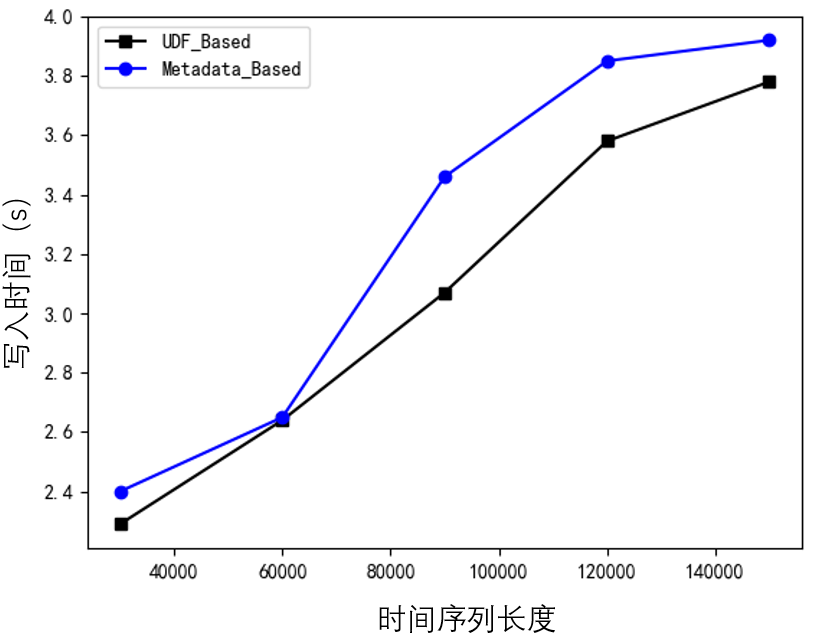
\includegraphics[width=0.49\linewidth]{truck_iotdb_write.png}}
  \subcaptionbox{挖掘机工况数据集\label{fig:excavator_write}}
  {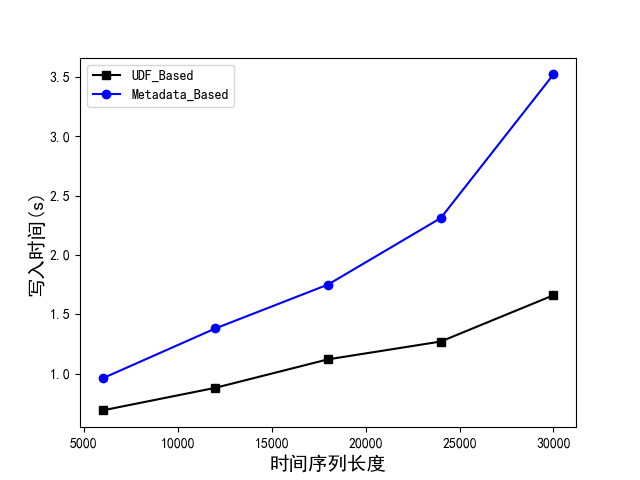
\includegraphics[width=0.49\linewidth]{excavator_iotdb_write.png}}
  \caption{不同数据量下基于UDF和基于元数据的算法写入性能对比}
  \label{fig:iotdb_write}
\end{figure}

\begin{figure}
  \centering
  \subcaptionbox{运输车GPS轨迹数据集\label{fig:truck_query}}
  {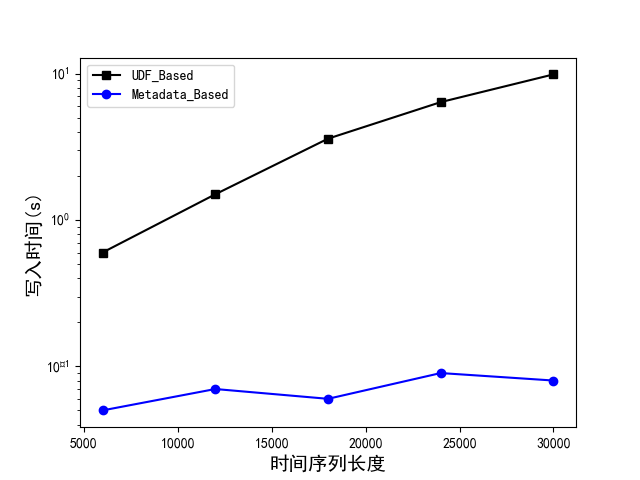
\includegraphics[width=0.49\linewidth]{truck_iotdb_query.png}}
  \subcaptionbox{挖掘机工况数据集\label{fig:excavator_query}}
  {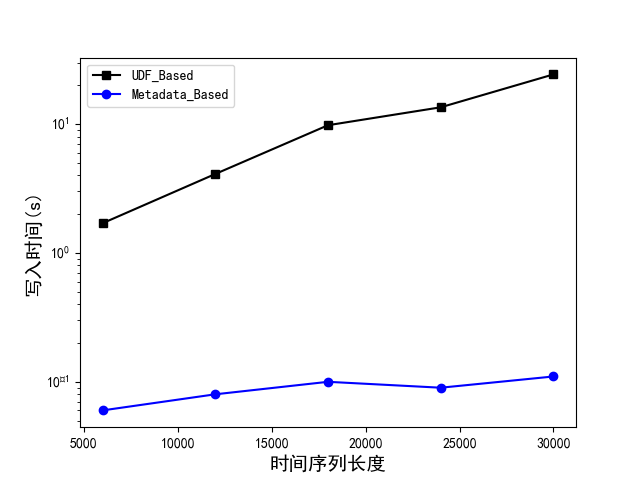
\includegraphics[width=0.49\linewidth]{excavator_iotdb_query.png}}
  \caption{不同数据量下基于UDF和基于元数据的算法查询性能对比}
  \label{fig:iotdb_query}
\end{figure}

本节在运输车GPS轨迹数据集和挖掘机
工况数据集上对基于UDF和基于元数据的对称子段挖掘算法实现
的写入和查询性能进行了实验,实验结果如图~\ref{fig:iotdb_write}
和~\ref{fig:iotdb_query}所示。
从图中可以看出,尽管基于元数据的分段算法写入性能略有下降,
但其查询分析性能却是基于UDF算法的数十倍。证明了基于
元数据的分段算法在查询负载较重的场景中具有重要的研究价值。

\section{本章小结}
本章使用了八个不同的数据集对第3章和第4章设计的对称子段判定和挖掘算法进行了
实验效果和性能评估。实验主要分为两类,首先是在四个UCR公开的数据集上
进行了对称子段判定效果的评估实验,结果证明无论数据集
是否具有对称性,本文设计的对称子段判定算法在综合评价指标
F值上均远远优于其他算法,能兼顾准确和完整地判定出所有的对称子段。
其次在一个合成数据集和三个真实工业与金融业场景中采集生成的数据集上
对对称子段挖掘算法的效果和时间效率进行评估,结果证明基于最优匹配
的对称子段挖掘算法在挖掘偏差率上远远低于基于一一对应匹配的挖掘算法。
而尽管基于动态时间扭曲的算法同样具有较低的挖掘偏差率,但其时间效率却比
对称子段挖掘算法低了100多倍。并且,结合IoTDB系统的存储和计算框架,
本章对基于UDF和元数据的分段算法的写入和查询性能进行了对比实验,
证明了基于UDF的实现适用于写入负载较重而基于元数据的实现适用于
查询负载较重的结论。
